\documentclass[11pt,oneside,english]{book}
\usepackage[T1]{fontenc}
\usepackage[latin1]{inputenc}
\usepackage{geometry}
\geometry{verbose,letterpaper,tmargin=1in,bmargin=1in,lmargin=1in,rmargin=1in}
\usepackage{babel}
\setcounter{secnumdepth}{3}
\setlength\parskip{\medskipamount}
\setlength\parindent{0pt}
\usepackage{url}
\usepackage[dvips]{graphicx}

\newcommand{\Erlang}            % Write Erlang correctly
        {{\sc Erlang}}


\newcommand{\Yaws}            % Write Erlang correctly
        {{\sc Yaws}}


\makeatletter

\usepackage[T1]{fontenc}
\usepackage{xspace}
\usepackage{html}

\makeatother
\begin{document}



\title{Yaws - Yet Another Web Server}


\author{Claes Wikstrom\\
klacke@hyber.org}





\maketitle
\tableofcontents{}



\chapter{Introduction}


\begin{figure}[h]
\begin{center}

 
\includegraphics[scale=0.6] {yaws_head.eps}

\end{center}           
\end{figure}    

\Yaws\  is an \Erlang\  web server. It's written in \Erlang\  and it uses
\Erlang\  as its embedded language similar to PHP in Apache or Java in Tomcat.

The advantages of \Erlang\  as an embedded web page language as opposed to
Java or PHP are many.
\begin{itemize}

\item{Speed - Using \Erlang\  for both implementing the web server itself as well
as embedded script language gives excellent dynamic page generation
performance.}

\item{Beauty - Well this is subjective}

\item{Scalability - due to the light weight processes of \Erlang\ , \Yaws\ 
is able to handle a very large number of concurrent connections}

\end{itemize}

\Yaws\  has a wide feature set, it supports:

\begin{enumerate}
\item HTTP 1.0 and HTTP 1.1 
\item Static content page delivery
\item Dynamic content generation using embedded \Erlang\  code in the
HTML pages
\item Common Log Format traffic logs
\item Virtual hosting with several servers on the same IP address
\item Multiple servers on multiple IP addresses.
\item HTTP tracing for debugging
\item An interactive interpreter environment in the Web server while
developing and debugging the web site.
\item RAM caching of commonly accessed pages.
\item Full streaming capabilities of both up and down load of dynamically
generated pages.
\item SSL 
\item Support for WWW-Authenticated pages.
\item Support API for cookie based sessions.
\item Application Modules where virtual directory hierarchies can
be made.
\item Embedded mode
\end{enumerate}

\section{Prerequisites}
This document requires that the reader:
\begin{itemize}
\item Is well acquainted with the \Erlang\  programming language
\item Understands basic Web technologies.
\end{itemize}


\section{A tiny example}

We introduce \Yaws\  by help of a tiny example. 
 The web server \Yaws\  serves  and delivers
static content pages similar to any old web server, except that \Yaws\  does this 
much faster than most web servers. It's the dynamic pages
that makes \Yaws\  interesting. Any page with the suffix ``.yaws'' is considered
a dynamic \Yaws\  page. A \Yaws\  page can contain embedded \Erlang\  snippets that
are executed while the page is being delivered to the WWW browser.

Example 1.1 is the HTML code for a small \Yaws\  page.


\begin{figure}[h]
\begin{verbatim}
<html>

<p> First paragraph

<erl>
out(Arg) ->
    {html, "<p>This string gets inserted into HTML document dynamically"}.
</erl>

<p> And here is some more HTML code

</html>
\end{verbatim}
\caption{Example 1.1}
\end{figure}

It illustrates the basic idea behind \Yaws\ . The HTML code
can contain <erl> and </erl> tags and inside these tags an \Erlang\  function
called out/1 gets called and the output of that function is inserted
into the HTML document, dynamically. 

It is possible to have several chunks of HTML code together with several 
chunks of \Erlang\  code in the same \Yaws\  page.

The \verb+Arg+ argument supplied to the automatically invoked \verb+out/1+
function is an \Erlang\  record that contains various data which is interesting 
when generating dynamic pages. For example the HTTP headers which were sent
from the WWW client, the actual TCP/IP socket leading to the WWW client.
This will be elaborated on throughly in later chapters. 

The \verb+out/1+ function returned the tuple \verb+{html, String}+ and 
\verb+String+ gets inserted into the HTML output. There are number
of different return values that can be returned from the \verb+out/1+ function
in order to control the behavior and output from the \Yaws\  web server.



\chapter{Compile, Install, Config and Run}

This chapter is more of a ``Getting started'' guide than a full
description of the \Yaws\  configuration. 
\Yaws\  is hosted on Sourceforge at 
\textit { http://sourceforge.net/projects/erlyaws/ }. This is where the source code
resides in a CVS repository and the latest unreleased version is
available through anonymous CVS through the following commands:

\begin{verbatim}

# export CVS_RSH=ssh 
# export CVSROOT=:pserver:anonymous@cvs.erlyaws.sourceforge.net:/cvsroot/erlyaws
# cvs  login
# cvs -z3 co .

\end{verbatim}


Released version of \Yaws\  are available either at the Sourceforge site or
at \textit{http://yaws.hyber.org/download}. 



\subsection{Compile and Install}

To compile and install a \Yaws\  release
one of the prerequisites is a properly installed \Erlang\  system. \Yaws\ 
runs on \Erlang\  releases OTP R8 and later. Get \Erlang\  from
\textit{http://www.erlang.org}

Compile and install is straight forward:
\begin{verbatim}
# cd /usr/local/src
# tar xfz yaws-X.XX.tar.gz
# cd yaws
# ./configure && make 
# make install
\end{verbatim}

The make command will compile the \Yaws\  web server with the \verb+erlc+
compiler found by the configure script.

make install - will install the executable - called \verb+yaws+ in
/usr/local/bin/ and a working configuration file in \textit{ /etc/yaws.conf}

make local\_install will install the executable in \$HOME/bin and a
working configuration file in \$HOME/yaws.conf

While developing a \Yaws\  site, it's typically most convenient to
use the local\_install and run \Yaws\  as a non privileged user.


\subsection{Configure}
Let's take a look at the config file that gets written to \$HOME after
a local\_install.


\begin{figure}[h]
\begin{verbatim}

# first we have a set of globals

logdir = .
ebin_dir = /home/klacke/yaws/yaws/examples/ebin
include_dir = /home/klacke/yaws/yaws/examples/include

# and then a set of servers

<server localhost>
        port = 8000
        listen = 127.0.0.1
        docroot = /home/klacke/yaws/yaws/scripts/../www
</server>


\end{verbatim}
\caption{Minimal Local Configuration}
\end{figure}

The configuration consists of an initial set of global
variables that are valid for all defined servers.

The only global directive we need to care about for now is the logdir. 
\Yaws\  produces a number of log files and they will -
using the Configuration from Figure 2.1 - end up in the current 
working directory.
We start \Yaws\  interactively as 
\begin{verbatim}
# ~/bin/yaws -i
Erlang (BEAM) emulator version 5.1.2.b2 [source]

Eshell V5.1.2.b2  (abort with ^G)
1> 
=INFO REPORT==== 30-Oct-2002::01:38:22 ===
Using config file /home/klacke/yaws.conf
=INFO REPORT==== 30-Oct-2002::01:38:22 ===
Listening to 127.0.0.1:8000 for servers ["localhost:8000"]

1>
\end{verbatim}

By starting \Yaws\  in interactive mode (using the command switch \textit{-i}
we get a regular \Erlang\  prompt. This is most convenient when developing
\Yaws\ /http pages. For example we:
\begin{itemize}
\item{Can dynamically compile and load optional helper modules we need.}
\item{Get all the crash and error reports written directly to the
terminal.}
\end{itemize}

The configuration in Example 2.1 defined one HTTP server on
address 127.0.0.1:8000 called "localhost".
It is important to understand the difference between the name and
the address of a server. The name is the expected value in the
client Host: header. That is typically the same as the fully qualified
DNS name of the server whereas the address is the actual 
IP address of the server.

Since \Yaws\  support virtual hosting with several servers on the same
IP address, this matters.

Nevertheless, our server listens to \textit{127.0.0.1:8000} and 
has the name "localhost", thus the correct URL for this server
is \textit{http://localhost:8000}.

The document root (docroot) for the server is set to the www directory in the
\Yaws\  source code distribution. This directory contains a bunch of
examples and we should be able to run all those example now on the
URL  \textit{http://localhost:8000}.

Instead of editing and adding files in the \Yaws\  www directory, we 
create yet another server on the same IP address but a different port
number - and in particular a different document root where we can add
our own files.

\begin{verbatim}
# mkdir ~/test
# mkdir ~/test/logs
\end{verbatim}

Now change the config so it looks like this:

\begin{verbatim}

logdir = /home/klacke/test/logs
ebin_dir = /home/klacke/test
include_dir = /home/klacke/test

<server localhost>
        port = 8000
        listen = 127.0.0.1
        docroot = /home/klacke/yaws/yaws/www
</server>

<server localhost>
        port = 8001
        listen = 127.0.0.1
        docroot = /home/klacke/test
</server>


\end{verbatim}

We define two servers, one being the original default
and a new pointing to a document root in our home directory.

We can now start to add static content in the form of
HTML pages, dynamic content in the form of .yaws pages or
\Erlang\ .beam code that can be used to generate the dynamic content.

The load path will be set so that beam code in the directory \verb+~/test+
will be automatically loaded when referenced.

It is best to run \Yaws\  interactively while developing the site.
In order to start the \Yaws\  as a daemon, we give the flags:
\begin{verbatim}
# yaws -D -heart
\end{verbatim}

The \textit{-D} flags instructs \Yaws\  to run as a daemon and the 
\textit{-heart} flags will start a heartbeat program called heart
which restarts the daemon if it should crash or if it stops responding to
a regular heartbeat.

Once started in daemon mode, we have very limited ways of interacting
with the daemon. It is possible to query the daemon using:
\begin{verbatim}
# yaws -S
\end{verbatim}

This command produces a simple printout of Uptime and number of hits
for each configured server.

If we change the configuration, we can HUP the daemon using the
command:
\begin{verbatim}
# yaws -h
\end{verbatim}

This will force the daemon to reread the configuration file.



\chapter{Static content}

\Yaws\  acts very much like any regular web server while delivering
static pages. By default \Yaws\  will cache static content in RAM.
The caching behavior is controlled by a number of global
configuration directives. Since the RAM caching occupies memory, 
it may be interesting to tweak the default values for the caching directives
or even to turn it off completely.

The following configuration directives control the caching behavior
\begin{itemize}
\item \textit{max\_num\_cached\_files = Integer}
\Yaws\   will  cache  small  files  such  as  commonly
              accessed  GIF images in RAM.  This directive sets a
              maximum number on the number of cached files.   The
              default value is 400.

\item\textit{max\_num\_cached\_bytes = Integer}
 This  directive  controls  the  total amount of RAM
             which can maximally be used for cached  RAM  files.
              The default value is 1000000, 1 megabyte.


\item\textit{max\_size\_cached\_file = Integer}

 This  directive  sets  a  maximum size on the files
              that are RAM cached by \Yaws\ .  The default  value  i
              8000, 8 batters.



\end{itemize}

It may be considered to be confusing, but the numbers specified 
in the above mentioned cache directives are local to each
server. Thus if we have specified \verb+max_num_cached_bytes = 1000000+
and have defined 3 servers, we may actually use $3 * 1000000$ bytes.




\chapter{Dynamic content}

Dynamic content is what \Yaws\  is about. Most web servers are designed
with HTTP and static content in mind whereas \Yaws\  is designed 
for dynamic pages from the start.
Most large sites on the Web today make heavy use of dynamic pages.



\section{Introduction}

When the client GETs a a page that has a .yaws suffix. The \Yaws\  server
will read that page from the hard disk and divide it in parts
that consist of HTML code and \Erlang\  code. Each chunk of \Erlang\  code
will be compiled into a module. The chunk of \Erlang\  code must contain
a function \verb+out/1+. If it doesn't the \Yaws\  server will insert a
proper error message into the generated HTML output.

When the \Yaws\  server ships a .yaws page it will process it chunk by chunk
through the .yaws file. If it is HTML code, the server will ship that
as is, whereas if it is \Erlang\  code, the \Yaws\  server will invoke the
\verb+out/1+ function in that code and insert the output of that \verb+out/1+ function into the stream
of HTML that is being shipped to the client.

\Yaws\  will (of course) cache the result of the compilation
and the next time a client requests the same .yaws page \Yaws\  will
be able to invoke the already compiled modules directly.


\section{EHTML}

There are two ways to make the \verb+out/1+ function generate HTML
output. The first and most easy to understand is by returning a tuple
\verb+{html, String}+ where \verb+String+ then is regular HTML data
(possibly as a deep list of strings and/or binaries) which will simply
be inserted into the output stream.
An example:

\begin{verbatim}
<html>
<h1> Example 1 </h1>

<erl>
out(A) ->
    Headers = A#arg.headers,
    {html, io_lib:format("You say that you're running ~p",
                         [Headers#headers.user_agent])}.

</erl>

</html>

\end{verbatim}


The second way to generate output is by returning a tuple
\verb+{ehtml, EHTML}+. The term \verb+EHTML+ must adhere to the 
following structure:

$EHTML = [EHTML] | \{TAG, Attrs, Body\} | 
                   \{TAG, Attrs\} | \{TAG\} |
        binary() | character()$

$TAG         = atom()$

$Attrs = [\{HtmlAttribute, Value\}]$

$HtmlAttribute   = atom()$

$Value = string() | atom()$

$Body  = EHTML$

We give an example to show what we mean:
The tuple 
\begin{verbatim}
{ehtml, {table, [{bgcolor, grey}],
         [
          {tr, [], 
           [
            {td, [], "1"},
            {td, [], "2"},
            {td, [], "3"}
           ],
           {tr, [],
            [{td, [{colspan, "3"}], "444"}]}}]}}.
\end{verbatim}

Would be expanded into the following HTML code
\begin{verbatim}
<table bgcolor="grey">
  <tr>
    <td> 1 </td
    <td> 2 </td>
    <td> 3 </td>
  </tr>
  <tr>
    <td colspan="3"> 444 </td>
  </tr>
</table>

\end{verbatim}

At a first glance it may appears as if the HTML code is more
beautiful than the \Erlang\  tuple. That may very well be the
case from a purely aesthetic point of view. However the
\Erlang\  code has the advantage of being perfectly indented by editors
that have syntax support for \Erlang\  (read Emacs). Furthermore, the \Erlang\ 
code is easier to manipulate from an \Erlang\  program.

As an example of some more interesting ehtml we could have
an \verb+out/1+ function that prints some of the HTTP headers.

In the www directory of the \Yaws\  source code distribution we have
a file called \verb+arg.yaws+. The file demonstrates the Arg \#arg record
parameter which is passed to the \verb+out/1+ function.


But before we discuss that code, we describe the Arg record  
in detail.

Here is the \verb+yaws_api.hrl+ file which is in included by default
in all \Yaws\ files. The \#arg{} record contains many fields that are
useful when processing HTTP request dynamically.
We have access to basically all the information which associated to the
client request such as:
\begin{itemize}

\item The actual socket leading back to the HTTP client
\item All the HTTP headers - parsed into a \#headers record.
\item The HTTP request - parsed into a \#http\_request record
\item clidata - Data which is POSTed by the client
\item querydata - This is the remainder of the URL following the first 
occurrence of a ? character - if any.
\item docroot - The absolute path to the docroot of the virtual server
that is processing the request.
\end{itemize}



\begin{verbatim}


-record(arg, {
          clisock,        %% the socket leading to the peer client
          headers,        %% headers
          req,            %% request
          clidata,        %% The client data (as a binary in POST requests)
          querydata,      %% Was the URL on the form of ...?query (GET reqs)
          appmoddata,     %% the remainder of the path leading up to the query
          docroot,        %% where's the data
          fullpath,       %% full path to yaws file
          cont,           %% Continuation for chunked multipart uploads
          state,          %% State for use by users of the out/1 callback
          pid,            %% pid of the yaws worker process
          opaque          %% useful to pass static data
         }).              


-record(http_request, {method,
                       path,
                       version}).

            
-record(headers, {
          connection,
          accept,
          host,
          if_modified_since,
          if_match,
          if_none_match,
          if_range,
          if_unmodified_since,
          range,
          referer,
          user_agent,
          accept_ranges,
          cookie = [],
          keep_alive,
          content_length,
          content_type,
          authorization,
          other = []   %% misc other headers
         }).

\end{verbatim}


There are a number of \textit{advanced} fields in the \#arg record
such as \verb+appmod+, \verb+opaque+ that will be discussed in later chapters.

Now, we show some code which displays the content of the Arg \#arg record.
The code is available in yaws/www/arg.yaws and after a a \verb+local_install+
a request to \textit{http://localhost:8000/arg.yaws} will run the code.

\begin{verbatim}

<html>

<h2> The Arg </h2>

<p>This page displays the Arg #argument structure
supplied to the out/1 function.

<erl>


out(A) ->
    Req = A#arg.req,
    H = yaws_api:reformat_header(A#arg.headers),
    {ehtml,
     [{h4,[], "The headers passed to us were:"},
      {hr},
      {ol, [],lists:map(fun(S) -> {li,[], {p,[],S}} end,H)},

      {h4, [], "The request"},
      {ul,[],
       [{li,[], f("method: ~s",  [Req#http_request.method])},
        {li,[], f("path: ~p",    [Req#http_request.path])},
        {li,[], f("version: ~p", [Req#http_request.version])}]},

      {hr},
      {h4, [], "Other items"},
      {ul,[],
       [{li,[], f("clisock from: ~p", [inet:peername(A#arg.clisock)])},
        {li,[], f("docroot: ~s",      [A#arg.docroot])},
        {li,[], f("fullpath: ~s",     [A#arg.fullpath])}]},
      {hr},
      {h4, [], "Parsed query data"},
      {pre,[], f("~p", [yaws_api:parse_query(A)])},
      {hr},
      {h4,[], "Parsed POST data "},
      {pre,[],  f("~p", [yaws_api:parse_post(A)])}]}.

</erl>

</html>

\end{verbatim}


The code utilizes 4 functions from the \verb+yaws_api+ module.
\verb+yaws_api+ is a general purpose www api module that contains various
functions that are handy while developing \Yaws\  code. We will see many 
more of those functions during the examples in the following chapters.

The functions used are:
\begin{itemize}
\item \verb+yaws_api:f/2+ alias for io\_lib:format/2. The \verb+f/1+ function
is automatically \verb+-includeed+ in all \Yaws\  code.
\item \verb+yaws_api:reformat_header/1+ - This function takes the \#headers record
and unparses it, that is reproduces regular text.
\item \verb+yaws_api:parse_query/1+ - The topic of next section.
\item \verb+yaws_api:parse_post/1+ -- Ditto.
\end{itemize}


\section{POSTs}

\subsection{Queries}

The user can supply data to the server in many ways. The most
common is to give the data in the actual URL.
If we invoke: 

\verb+GET http://localhost:8000/arg.yaws?kalle=duck&goofy=unknown+

we pass two parameters to the \textit{arg.yaws} page.
That data is URL-encoded by the browser and the server can retrieve the
data by looking at the remainder of the URL following the ? character.
If we invoke the \verb+arg.yaws+ page with the above mentioned URL we get
as the result of \verb+yaws_parse_query/1+:

$kalle = duck$

$goofy = unknown$

In \Erlang\  terminology, the call \verb+yaws_api:parse_query(Arg)+ returns
the list: 
\begin{verbatim}
[{kalle, "duck"}, {goofy, "unknown"}]
\end{verbatim}

Note that the first element is transformed into an atom, whereas the value
is still a string.

hence, a web page can contain URLs with a query and thus pass data to the
web server. This scheme works both with GET and POST requests.
It is the easiest way to pass data to the Web server since no FORM is required
in the web page.


\subsection{Forms}

In order to POST data a FORM is required, say that we have a page called
\verb+form.yaws+ that contain the following code:

\begin{verbatim}
<html>
<form action="/post_form.yaws"
      method="post"

<p> A Input field
<input name="xyz" type="text">
<input type="submit">
</form>
</html>
\end{verbatim}
 
This will produce a page with a simple input field and a Submit button.



\begin{figure}[h]
\begin{center}

 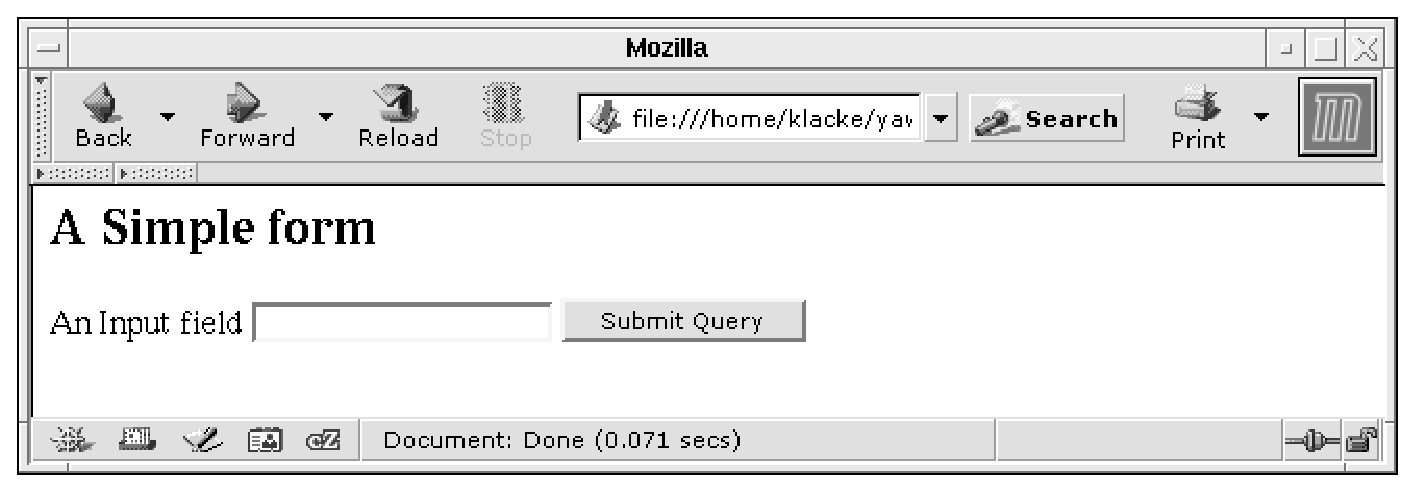
\includegraphics[scale=0.6] {a.eps}

\end{center}           
\end{figure}    
 


If we enter something - say ``Hello there `` - 
in the input field and click the Submit button the
client will request the page indicated in the ``action'' attribute, namely
\verb+post_form.yaws+.


If that \Yaws\  page has the following code:
\begin{verbatim}
out(A) ->
   L = yaws_api:parse_post(A),
   {html, f("~p", [L])}
\end{verbatim}

The user will see the output
\begin{verbatim}
[{xyz, "Hello there"}]
\end{verbatim}

The differences between using the query part of the URL
and a form are the following:
\begin{itemize}
\item Using the query arg only works in GET request. We parse the
query argument with the function \verb+yaws_api:parse_query(Arg)+

\item If we use a form and POST the user data the client will
transmit the user data in the body of the request.
That is - the client sends a request to get the page using the POST method
and it then attaches the user data - encoded - into the body of the
request.

A POST request can have a query part in its URL as well as user data 
in the body.
\end{itemize}


\section{POSTing files}

It is possible to upload files from the client to the server by
means of POST. We indicate this in the form by telling the browser that we
want a different encoding, here is a form that does this:
\begin{verbatim}

out(A) ->
    Form = 
        {form, [{enctype, "multipart/form-data"},
                {method, post},
                {action, "file_upload_form.yaws"}],
                [{input, [{type, submit}, {value, "Upload"}]},
                 {input, [{type,file}, {width, "50"}, {name, foo}]}]},
    {ehtml, {html,[], [{h2,[], "A simple file upload page"},
                      Form]}}.

\end{verbatim}

The page delivers the entire HTML page with enclosing \verb+html+ markers.
It looks like:


\begin{figure}[h]
\begin{center}

 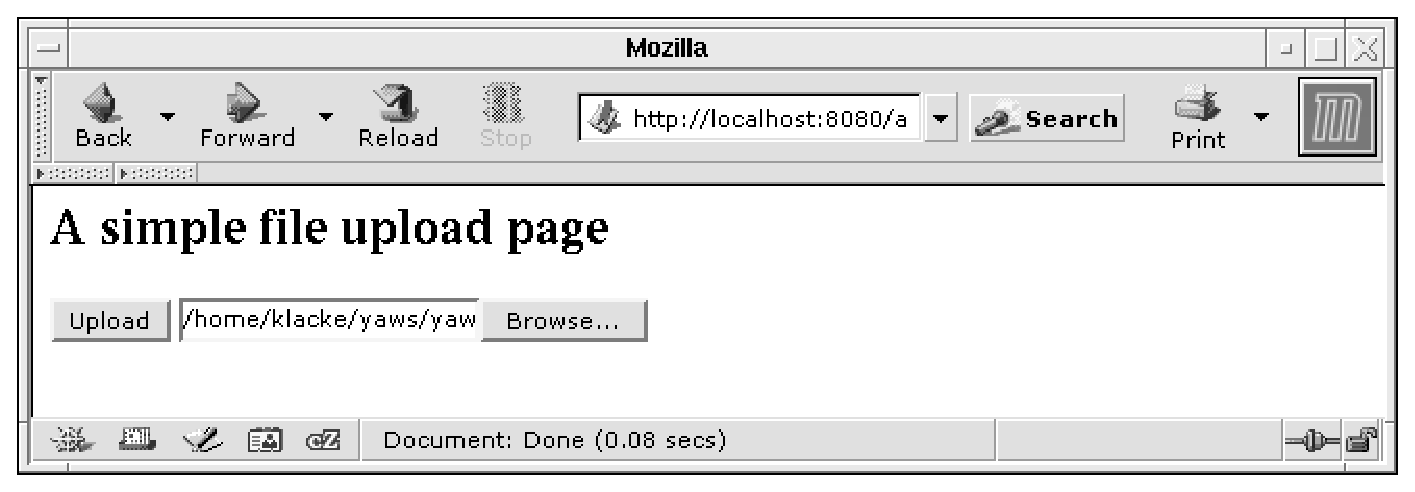
\includegraphics[scale=0.6] {b.eps} 

\end{center}           
\end{figure}    
 
The user get an option to browse the local host for a file
or the user can explicitly fill in the file name in the input
field. The file browsing part is automatically taken care of by the
browser.

The action field in the form states that the client shall POST to a page called
\verb+file_upload_form.yaws+. This page will get the contents of the file
in the body of the POST message. Here we have one easy case and one hard
case. \Yaws\  will read the data from the client. However if the file is large
the entire contents of the file will not be part of the read operation.
It is not acceptable to let \Yaws\  continue to read the full POST body
and then when that is done, invoke the POST page. \Yaws\  must
feed the page with the chunks of the file as they arrive.

First the easy case:

Not YET  Written ... .....  fill this in later .....





\chapter{Mode of operation}

\section{On the fly compilation}
When the client requests a \Yaws\  page, \Yaws\  will look in its caches
(there is one cache per virtual server) to see if it finds the
requested page in the cache. If \Yaws\  doesn't find the page in the
cache, it will compile the page. This only happens the first time a
page is requested.
Say that the page is 400 bytes big has the following layout:



\begin{figure}[h]
\begin{center}

 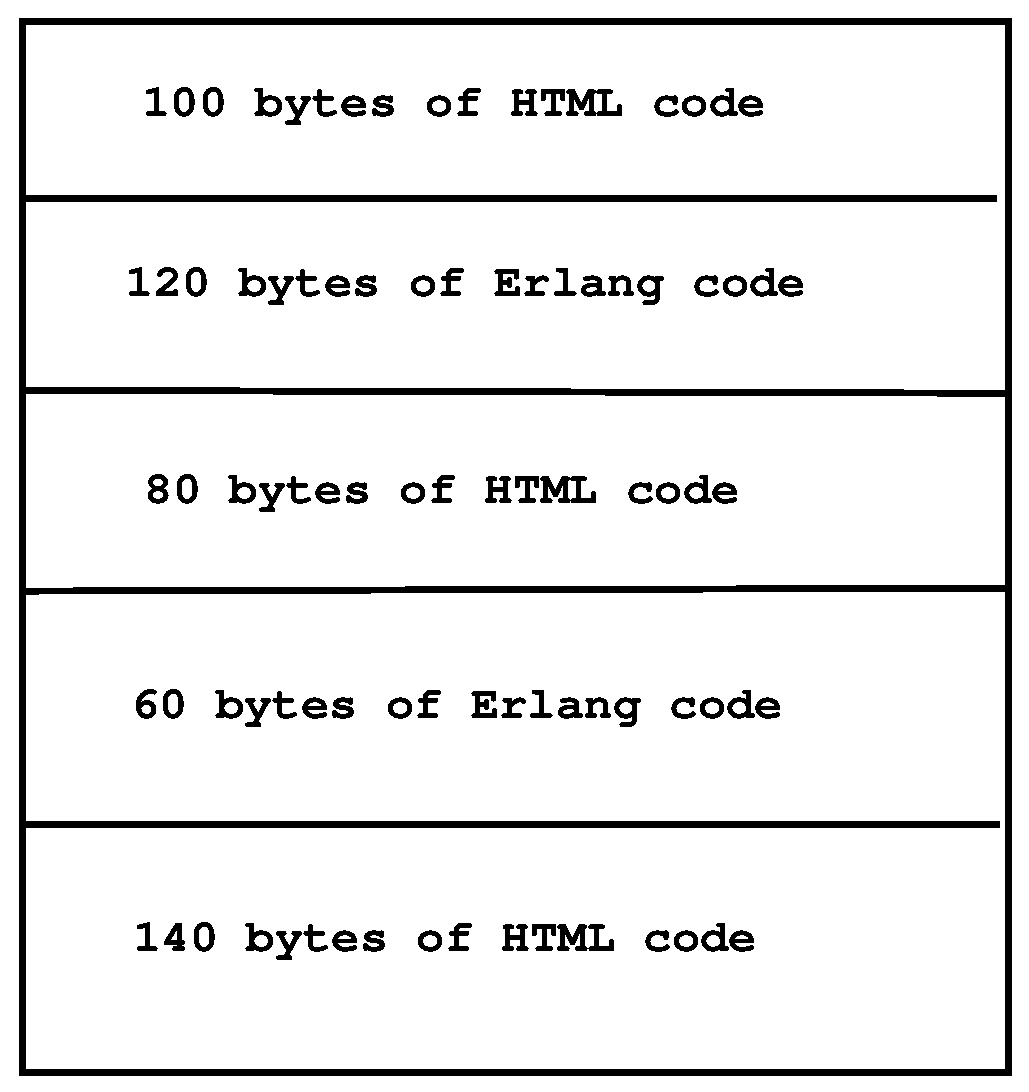
\includegraphics[scale=0.4] {layout.eps}

\end{center}           
\end{figure}    

The \Yaws\  server will then parse the file and produce a structure
which makes it possible to deliver the page in a readily fashion the
next time the same page is requested.

When shipping the page it will
\begin{enumerate}
\item Ship the first 100 bytes from the file
\item Evaluate the first \Erlang\  chunk in the file and ship the output
from the \verb+out/1+ function in that chunk. It will also jump ahead
in the file and skip 120 bytes.
\item Ship 80 bytes of HTML code 
\item Again evaluate an \Erlang\  chunk, this time the second and jump
ahead 60 bytes in the file.
\item And finally ship 140 bytes of HTML code to the client
\end{enumerate}

\Yaws\  writes the source output of the compilation into a directory
/tmp/yaws/\$UID. The beam files are never written to a file. 
Sometimes it can be useful to look at the generated source code
files, for example if the \Yaws\ /\Erlang\  code contains a compilation
error which is hard to understand.


\section{Evaluating the \Yaws\  code}

All client requests will execute in their own \Erlang\  process.
For each group of virtual hosts on the same IP:PORT pair
one \Erlang\  process listens for incoming requests. 

This process spawns acceptor processes for each incoming request.
Each acceptor process reads and parses all the HTTP headers from the
client. It then looks at the Host: header to figure out which 
virtual server to use, i.e. which docroot to use for this
particular request. If the Host: header doesn't match 
any server from \textit{yaws.conf} with that IP:PORT pair, the first
one from \textit{yaws.conf} is chosen.


By default \Yaws\  will not ship any data at all to the client
while evaluating a \Yaws\  page. The headers as well as the generated
content are accumulated and not shipped to the client until the 
entire page has been processed.



\chapter{SSL}

SSL - Secure Socket Layer is a protocol used on the Web for
delivering encrypted pages to the WWW client. SSL is widely deployed
on the Internet and virtually all bank transactions as well as all
on-line shopping today is done with SSL encryption. There are many
good sources on the net that describes SSL in detail - and I will not
try to do that here. 
There  is for example a good document at:
\verb+http://www.tldp.org/HOWTO/SSL-Certificates-HOWTO/+ which
describes how to manage certificates and keys.

In order to run an SSL server we must have a certificate. Either we
can create a so called self-signed certificate ourselves or buy a
certificate from one of the many CA's (Certificate Authority's) on the
net. \Yaws\  use the otp interface to openssl.

To setup a \Yaws\  server with SSL we could have a \textit{yaws.conf} file that
looks like:

\begin{verbatim}

 logdir = /var/log/yaws

<server www.funky.org>
               port = 443
               listen = 192.168.128.32
               docroot = /var/yaws/www.funky.org
               <ssl>
                  keyfile = /etc/funky.key
                  certfile = /etc/funky.cert
                  password = gazonk
               </ssl>
       </server>
\end{verbatim}

This is the easiest possible SSL configuration. The configuration
refers to a certificate file and a key file. The certificate file
must contain the name "www.funky.org" as it "Common Name".

The keyfile is the private key file and it is encrypted using
the password "gazonk".






\chapter{Applications}

\Yaws\  is well suited for Web applications. In this chapter we will
describe a number of application templates. Code and strategies that
can be used to build Web applications.

There are several ways of starting applications from
\Yaws\  . 

\begin{itemize}
\item The first and most easy variant is to specify
the \verb+-r Module+ flag to the \Yaws\  startup script.
This will \verb+apply(Module,start,[])+

\item We can also specify runmods in the \textit{yaws.conf} file.
It is possible to have several modules specified if want
the same \Yaws\  server to run several different applications.

\begin{verbatim}

runmod = myapp
runmod = app_number2

\end{verbatim}

\item It is also possible to do it the other way around, let 
the main application start \Yaws\ . We call this embedded mode 
and that will be discussed in a later chapter,

\end{itemize}



\section{Login scenarios}

Many Web applications require the user to login. Once the user has
logged in the server sets a Cookie and then the user will be
identified by help of the cookie in subsequent requests. 

  \subsection{The session server}
The cookie is passed in the headers and is available to the \Yaws\ 
programmer in the Arg \#arg record. The \Yaws\  session server
can help us to maintain a state for a user while the user is
logged in to the application. The session server has the following 5
api functions to aid us:

\begin{enumerate}

\item \verb+yaws_api:new_cookie_session(Opaque)+
This function initiates a new cookie based session. The Opaque data
is typically some application specific structure which makes it
possible for the application to read a user state, or it can be the
actual user state itself.

\item \verb+yaws_api:cookieval_to_opaque(Cookie)+
This function maps a cookie to a session.

\item \verb+yaws_api:replace_cookie_session(Cookie, NewOpaque)+
Replace the Opaque user state in the session server.

\item \verb+yaws_api:delete_cookie_session(Cookie)+
This function should typically be called when the user logs out
or when our web application decides to auto logout the user.

\end{enumerate}


All cookie based applications are different but they have 
some things in common. In the example that follow we assume the
existence of a function \verb+myapp:auth(UserName, Passwd)+ and it
returns \verb+ok+ or \verb+{error, Reason}+


Furthermore - let's have a record:

\begin{verbatim}

-record(session, {user,
                  passwd,
                  udata = []}).

\end{verbatim}

The following function is a good template function to 
check the cookie.


\begin{verbatim}

get_cookie_val(CookieName, Arg) ->
    H = Arg#arg.headers,
    yaws_api:find_cookie_val(CookieName, H#headers.cookie).



check_cookie(A, CookieName) ->
    case get_cookie_val(CookieName, A) of
        []  ->
            {error, "not logged in"};
        Cookie ->
            yaws_api:cookieval_to_opaque(Cookie)
    end.

\end{verbatim}


So what we need to do is the following: We want to check all
requests and make sure the the session\_server has our cookie registered as
an active session.

If a request comes in without a working cookie we want to present
a login page instead of the page the user requested.

Another quirky issue is that the pages necessary for display of the
login page must be shipped without checking the cookie.

  \subsection{Arg rewrite}

In this section we describe a feature whereby the user is allowed to
rewrite the Arg at an early stage in the \Yaws\  server.
We do that by specifying an \verb+arg_rewrite_mod+ in the \textit{yaws.conf} file.
\begin{verbatim}
arg_rewrite_mod = myapp
\end{verbatim}


Then in the \verb+myapp+ module we have:

\begin{verbatim}
arg_rewrite(Arg) ->
    OurCookieName = "myapp_sid"
    case check_cookie(A, OurCookieName) of
        {error, _} ->
            do_rewrite(Arg);
        {ok, _Session} ->
            %return Arg untouched
            Arg
    end.

%% these pages must be shippable without a good cookie
login_pages() ->
    ["/banner.gif", "/login.yaws", "/post_login.yaws"].

do_rewrite(Arg) ->
    Req = Arg#arg.req,
    {abs_path, Path} = Req#http_request.path,
    case lists:member(Path, login_pages()) of
        true ->
            Arg;
        false ->
            Arg#arg{req = Req#http_request{path = {abs_path, "/login.yaws"}},
                    state =  {abs_path, Path}}
    end.

\end{verbatim}

Our arg rewrite function lets all Args go through untouched 
that either have a good cookie or belong to a set of predefined
pages that are acceptable to get without being logged in.
If we decode that the user must log in,
 we change the path of the request,
 thereby making the \Yaws\  server ship a login page instead of the page the 
user requested. We also set the original path in the Arg state argument so
that the login page can redirect the user to the original page - once the login procedure is finished.



  \subsection{Authenticating}


Now we're approaching the \verb+login.yaws+ page, the page that displays
the login prompt to the user. The login page consists of two parts,
one part that displays the login data as a form and one form processing page
that reads the data the user entered in the login fields and performs
the actual authentication.

The login page performs a tiny well known Web trick where it
passes the original URL request in a hidden field in the login page and thereby passing that information to the form processing page.

The page \verb+login.yaws+:

\begin{verbatim}
<erl>

out(A) ->
    {ehtml,
     {html,[],
      [{h2, [], "Login page"},
       {hr},
       {form, [{action,"/login_post.yaws"},
               {method,post}],
        
        [{p,[], "Username"}, {input, [{type,text},{name,uname}]},
         {p,[],"Password"},  {input, [{type,password},{name,passwd}]},
         {input, [{type,submit},{value,"Login"}]},
         {input, [{type,hidden},{name,url}, 
                  {value, A#arg.state}]}]}]}}.

</erl>
\end{verbatim}



The form processing page which gets the POST data from the
code above looks like:
\begin{verbatim}


<erl>

-include("myapp.hrl").  
%% we have the session record there
%% we must set the include_path in the yaws.conf file
%% in order for the compiler to find that file

kv(K,L) ->
    {value, {K, V}} = lists:keysearch(K,1,L),
    V.
    
out(A) ->
    L = yaws_api:parse_post(A),
    User = kv(user, L),
    Pwd =  kv(passwd, L),
    case myapp:auth(User, Pwd) of
        ok ->
            S = #session{user = User,
                         passwd = Pwd,
                         udata = []},
            %% Now register the session to the session server
            Cookie = yaws_api:new_cookie_session(S),
            [{redirect_local, kv(url, L)},
              yaws_api:setcookie("myapp_sid",Cookie)]
        Err ->
            {ehtml, 
             {html, [],
              {p, [], f("Bad login: ~p",[Err])}}}
    end.

</erl>


    
\end{verbatim}

The function returns a list of two new previously not discussed return
values: Instead
of returning HTML output as in \verb+{html, Str}+ or
\verb+{ehtml,Term}+ 
we return a list of two new values. There are many different possible
return values from the \verb+out/1+ function and they will all be
described later. 

\begin{enumerate}

\item The tuple \verb+{redirect_local, Path}+. 
This particular redirect return value will make the 
\Yaws\  web server return a 303 redirect to the specified Path.

\item \verb+yaws_api:setcookie("myapp_sid",Cookie)+ generates
a \verb+Set-Cookie+ header
\end{enumerate}



Now if we put all this together we have a full blown cookie based
login system. The last thing we did in the form processing code was
to register the session with the session server thereby letting any
future requests go straight through the \verb+Arg+ rewriter.

This way both \Yaws\  pages as well as all or some static content
is protected by the cookie login code.


\subsection{Database driven applications}

We can use code similar to the code in the previous section to associate
a user session to entries in a database. Mneisa fits perfectly
together with \Yaws\  and keeping user persistent state in Mnesia is
both easy and convenient.

Once the user has logged in we can typically use the user name
as key into the database. We can mix ram\_tables and disc\_tables
to our liking. The Mneisa database must be initialized by means
of \verb+create_table/2+ before it
can be used. This is typically done while installing the
web application on a machine. 

Another option is to let the application check that Mnesia
is initialized whenever the application starts.

If we don't want or need to use Mnesia, it's of course possible
to use a simple \verb+dets+ file or a text file as well. 

\section{Appmods}

Appmods is mechanism to invoke different applications
based upon the URL. A URL - as presented to the web server in 
a request - has a path part and a query part.

It is possible to install several appmods in the \textit{yaws.conf}
file as:
\begin{verbatim}

appmods = foo myapp

\end{verbatim}

Now, if the user requests a URL where any component in the
directory path is an appmod, the parsing of the URL will terminate
there and instead of reading the actual file from the disk, \Yaws\  will
invoke the appmod with the remainder of the path inserted into
\verb+Arg#arg.appmoddata+.

Say the user requests the URL \textit{http://www.funky.org/myapp/xx/bar.html}
\Yaws\  will not ship the file \verb+bar.html+ to the client, instead it
will invoke \verb+myapp:out(Arg)+ with \verb+Arg#arg.appmoddata+
set to the string \verb+xx/bar.html+. Any optional query data - that
is data that follows the first "?" character in the URL - 
is removed from the path and passed as \verb+Arg#arg.querydata+.

Appmods can be used to run applications on a server. All requests
to the server that has an appmod in the URL will be handled by that
application. If the application decides that it want to 
ship a page from the disk to the client, it can return the
tuple \verb+{page, Path}+. This return value will make \Yaws\  read
the page from the disk, possibly add the page to it's cache of
commonly accessed pages and ship it back to the client.

The \verb+{page, Path}+ return value is equivalent to a
redirect, but it removes an extra round trip - and is thus faster.

Appmods can also be used to fake entire directory hierarchies
that doesn't exists on the disk. 


\section{The opaque data}

Sometimes an application needs application specific data
such as the location of its data files or whatever. There exists 
a mechanism to pass application specific configuration data from the
\Yaws\  server to the application. 

When configuring a server we have an opaque field in the
configuration file that can be used for this purpose.
Say that we have the following fields in the 
config file:
\begin{verbatim}

<server foo>
    listen = 192.168.128.44
    <opaque>
        foo = bar
        somefile = /var/myapp/db
        myname = hyber
    </opaque>
</server>
\end{verbatim}

This will create a normal server that listens to the specified IP address.
An application has access to the opaque data that was specified
in that particular server through \verb+Arg#arg.opaque+

If we have the opaque data specified above, the Arg opaque field will
have the value:

\begin{verbatim}

[{foo, "bar"}, 
 {somefile, "/var/myapp/db"},
 {myname, "hyber"}
]

\end{verbatim}





\section{Customizations}

When actually deploying an application at a live site, some
of the standard \Yaws\  behaviors are not acceptable. Many sites
want to customize the web server behavior when a client requests
a page that doesn't exists on the web server. The standard \Yaws\ 
behavior
is to reply with status code 404 and a message explaining that the
page doesn't exist.

Similarly, when \Yaws\  code crashes, the Reason for the crash is
displayed in the Web browser. This is very convenient while
developing a sit but not acceptable in production.


  \subsection{404 File not found}

We can install a special handler for 404 messages. We do that by
specifying a \verb+errormod_404+ in the \textit{yaws.conf} file.

If we have:

\begin{verbatim}
<server foo>
  ..
  ..
  ..
  errormod_404 = myapp

</server>

\end{verbatim}

When \Yaws\  gets a request for  a file that doesn't exists
on the hard disk, it invokes the errormod\_404 module
to generate both the status code as well as the content of the
message.

        \verb+Module:out404(Arg, GC, SC)+ will
                   be invoked by \Yaws\ . The arguments are

\begin{itemize}
\item              Arg is a \#arg{} record

\item              GC  is  a  \#gconf{}   record   (defined   in
              yaws.hrl)

\item              SC   is   a   \#sconf{}  record  (defined  in
              yaws.hrl)
\end{itemize}

              The function can and must do the same things
              that a normal \verb+out/1+ does.




  \subsection{Crash messages}

We use a similar technique for generating the crash messages, we
install a module in the \textit{yaws.conf} file and let that module generate
the crash message.
We have:
\begin{verbatim}
errormod_crash = Module
\end{verbatim}

The  default  is  to  display the
entire  formated  crash   message   in   the
browser.  This is good for debugging but not
in production.

The function \verb+Module:crashmsg(Arg,  SC,  Str)+
will  be  called.  The Str is the real crash
message formated as a string.



\section{Stream content}

If the \verb+out/1+ function returns the tuple
\verb+{content, MimeType, Content}+ \Yaws\  will
ship that data to the Client. This way we can
deliver dynamically generated content to the client
which is of a different mime type than "text/html".

If the generated file is very large and it not
possible to generate the entire file, we can
return the value:
\verb+{streamcontent, MimeType, FirstChunk}+ and then
from a different \Erlang\  process deliver the remaining chunks by using
the functions:
\begin{enumerate}
\item \verb+yaws_api:stream_chunk_deliver(YawsPid, Data)+
where the \verb+YawsPid+ is the process id of the \Yaws\  worker
process. That pid is available in \verb+Arg#arg.pid+

\item \verb+stream_chunk_end(YawsPid)+ This function
must be called to indicate the end of the stream.
\end{enumerate}


\section{All out/1 return values}

\begin{itemize}


\item       \verb+{html, DeepList}+
              This  assumes that DeepList is formatted HTML code.
              The code will be inserted in the page.

\item       \verb+{ehtml, Term}+
              This will transform the \Erlang\   term  Term  into  a
              stream of HTML content. 

\item       \verb+{content, MimeType, Content}+
              This function will make  the  web  server  generate
              different  content  than HTML. This return value is
              only allowed in a \Yaws\   file  which  has  only  one
              <erl> </erl> part and no html parts at all.

\item       \verb+{streamcontent, MimeType, FirstChunk}+
              This  return  value plays the same role as the con�
              tent return value above.  However it makes it  possible 
              to stream data to the client if the \Yaws\  code
              doesn't have access to all  the  data  in  one  go.
              (Typically  if  a  file  is  very  large or if data
              arrives from back end servers on the network.

\item       \verb+{header, H}+
              Accumulates a HTTP header. Used by for example  the
              \verb+yaws_api:setcookie/2-6+ function.

\item       \verb+{allheaders, HeaderList}+
              Will  clear  all previously accumulated headers and
              replace them.

\item       \verb+{status, Code}+
              Will set another HTTP status code than 200.

\item       \verb+break+  Will stop processing of any consecutive  chunks  of
              erl or html code in the \Yaws\  file.

\item       \verb+ok+     Do nothing.

\item       \verb+{redirect, Url}+
              Erase  all previous headers and accumulate a single
              Location header. Set the status code.

\item       \verb+{redirect_local, Path}+
              Does a redirect to the same Scheme://Host:Port/Path
              as we currently are executing in.

\item       \verb+{get_more, Cont, State}+
              When  we  are  receiving  large POSTs we can return
              this value and be  invoked  again  when  more  Data
              arrives.

\item       \verb+[ListOfValues]+
              It  is  possible  to  return  a  list  of the above
              defined return values.

\end{itemize}



\chapter{Debugging and Development}

\Yaws\  has excellent debugging capabilities. First and foremost we
have the ability to run the web server in interactive mode by means of
the command line switch \verb+-i+

This gives us a regular \Erlang\  command line prompt and we can
use that prompt to compile helper code or reload helper
code. Furthermore all error messages are displayed there.
If a .yaws page producees any regular \Erlang\ io, that output will
be displayed at the \Erlang\ prompt - assuming that we are running in interactive mode.

If we give the command line switch \verb+-d+ we get some
additional error messages. Also \Yaws\  does some additional checking
of user supplied data such as headers.

\section{Logs}
\Yaws\  produces various logs. All log files are written into the
\Yaws\  logdir directory. This directory is specified in the config file.

We have the following log files:
\begin{itemize}
\item The access log. Access logging is turn on or off per server
in the \textit{yaws.conf} file. If access\_log is turned on for a server,
\Yaws\  will produce a log in Common Access Log Format called
\textit{HostName:PortNumber.access}

\item \textit{report.log} This file contains all error and crash
messages for all virtual servers in the same file.

\item \textit{trace.traffic} and \textit{trace.http} The two
command line flags \verb+-t+ and \verb+-T+ tells \Yaws\  to trace 
all traffic or just all HTTP messages and write them to a file.
\end{itemize}



\chapter{Security}

\Yaws\  is of course susceptible to intrusions. \Yaws\  has the
ability to run under a different user than root - Assuming we need
to listen to privileged port numbers. Running as root is generally a
bad idea.  

Intrusions can happen basically at all places in \Yaws\  code where the
\Yaws\  code calls either the BIF \verb+open_port+ or when \Yaws\  code
does calls to \verb+os:cmd/1+.

Both \verb+open_port+ and \verb+os:cmd/1+ invoke the \verb+/bin/sh+
interpreter to execute its commands. If the commands are nastily
crafted bad things can easily happen.

All data that is passed to these two function must be carefully
checked.

Since \Yaws\  is written in \Erlang\  a large class of cracks are
eliminated since it is not possible to perform any buffer overrun
cracks on a \Yaws\  server. This is very good.


Another possible point of entry to the system is by providing a URL
which takes the client out from the docroot. This should not be
possible - and the impossibility relies on the correctness of the URL
parsing code in \Yaws\ . 

\section{WWW Authenticate}
\Yaws\  has support for WWW authenticate protected directories.
The access rights to different directories is controlled by directives
in the \textit{yaws.conf} file.

We can specify several auth groups in a server configuration.
If we have the following in the \textit{yaws.conf} file:


\begin{verbatim}

<server foo>
..
..

  <auth>
    realm = secretpage
    dir = /var/yaws/www/protected
    user klacke:gazonk
    user jonny:xyz
    user ronny:12r8uyp09jksfdge4
  </auth>
</server>
\end{verbatim}



\Yaws\  will protect all files in the specified directory by means
of WWW-Authenticate  access. If a user requests a page in the
directory, and doesn't have the correct WWW-Authenticate header, \Yaws\ 
will reply with a proper status code that makes the browser pop up a
login window.


\chapter {Embedded mode}

\Yaws\  is a normal OTP application. It is possible to integrate \Yaws\ 
into another - larger - application. The \Yaws\  source tree must be
integrated into the larger applications build environment. \Yaws\  is
then simply started by \verb+application:start()+ from the larger
applications boot script.

By default \Yaws\  reads its configuration data from a config file, the
default is "/etc/yaws.conf". If \Yaws\  is integrated into a larger
application that application typically has its configuration data kept
at some other centralized place. Sometimes we may not even have a file
system to read the configuration from if we run a small embedded
system.

\Yaws\  reads its application environment. If the environment key
\verb+embedded+ is set to t\verb+true+, \Yaws\  starts in embedded mode.
Once started it must be fed a configuration, and that can be done
after \Yaws\  has started by means of the function
\verb+yaws_api:setconf/2+.

It is possible to call \verb+setconf/2+ several times to force \Yaws\  to
reread the configuration.




\chapter{The config file - yaws.conf}

In this section we provide a complete listing of all possible
configuration file options.
The
       configuration contains two distinct parts  a  global  part
       which  affects  all  the  virtual  hosts and a server part
       where options for each virtual host is supplied.

\section{Global Part}

\begin{itemize}


\item       \verb+dir = Directory+ -
              All \Yaws\  logs will be  written  to  files  in  this
              directory.  There  are  several different log files
              written by \Yaws\ .

              \begin{itemize}
              \item report.log - this is a text file that contains  all
              error logger printouts from \Yaws\ .
              \item Host.access - for each virtual host served by \Yaws\ ,
              a file Host.access will be written  which  contains
              an access log in Common Log Format.
              \item trace.http  -  this file contains the HTTP trace if
              that is enabled
              \item trace.traffic -  this  file  contains  the  traffic
              trace if that is enabled
              \end{itemize}

\item        \verb+ebin_dir = Directory+ -
              This  directive adds Directory to the \Erlang\  search
              path. It is possible to have several of these  command 
              in the configuration file.

\item        \verb+include_dir = Directory+ -
              This directive adds Directory to the path of directories  
               where  the  \Erlang\   compiler  searches  for
              include  files.  We  need to use this if we want to
              include .hrl files in our \Yaws\  \Erlang\  code.

\item        \verb+max_num_cached_files = Integer+ -
              \Yaws\   will  cache  small  files  such  as  commonly
              accessed  GIF images in RAM.  This directive sets a
              maximum number on the number of cached files.   The
              default value is 400.

\item        \verb+max_num_cached_bytes = Integer+ -
              This  directive  controls  the  total amount of RAM
              which can maximally be used for cached  RAM  files.
              The default value is 1000000, 1 megabyte.

\item        \verb+max_size_cached_file = Integer+ -
              This  directive  sets  a  maximum size on the files
              that are RAM cached by \Yaws\ .  The default  value  i
              8000, 8 kBytes.

\item        \verb+cache_refresh_secs = Integer+
              The  RAM  cache  is used to serve pages that sit in
              the  cache.  An  entry  sits  in  cache   at   most
              cache\_refresh\_secs  number  of seconds. The default
              is 30. This means that when the content is  updated
              under  the  docroot, that change doesn't show until
              30 seconds have passed.  While  developing  a  \Yaws\ 
              site,  it may be convenient to set this value to 0.
              If the debug flag (-d) is passed to the \Yaws\   start
              script, this value is automatically set to 0.

\item        \verb+trace  = traffic | http+ -
              This  enables  traffic  or http tracing. Tracing is
              also possible to enable with a command line flag to
              \Yaws\ .

\item        \verb+username  = User+ -
             When Yaws is run as root, it can be configured to 
             change userid once it has created the necessary
	     listen sockets on privilged ports.


\end{itemize}



\section{Server Part}

\Yaws\   can  virthost  several  web servers  on  the  same IP
       address as well as  several  web servers  on  different  IP
       addresses.  The  on  limitation  here is that there can be
       only one server with ssl enabled per  each  individual  IP
       address.   Each virtual host is defined within a matching
       pair of \verb+<server ServerName>+ and \verb+</server>+. 
       The  ServerName
       will be the name of the web server.

       The following directives are allowed inside a server definition.

\begin{itemize}




\item              \verb+port = Port+ -
              This makes the server listen on Port

\item        \verb+listen = IpAddress+ -
              This makes the  server  listen  on  IpAddress  When
              virthosting  several  servers  on  the same IP/port
              address, if the browser doesn't send a Host: field,
              \Yaws\   will  pick  the first server specified in the
              config file

\item       \verb+rport = Port+
              This forces  all  local  redirects  issued  by  the
              server  to  go  to  Port.  This is useful when \Yaws\ 
              listens to a port which is different from the  port
              that  the  user  connects  to. For example, running
              \Yaws\  as a non-privileged user makes  it  impossible
              to  listen  to port 80, since that port can only be
              opened by a privileged user. Instead  \Yaws\   listens
              to  a high port number port, 8000, and iptables are
              used to redirect traffic to port 80  to  port  8000
              (most NAT:ing firewalls will also do this for you).

\item       \verb+rscheme = http | https+
              This forces  all  local  redirects  issued  by  the
              server  to  use this method. This is useful when an
              SSL off-loader, or stunnel, is  used  in  front  of
              \Yaws\ .

\item       \verb+access_log = true | false+
              Setting  this  directive  to  false turns of
              traffic logging for this virtual server. The
              default value is true.

\item               \verb+docroot  =  Directory+ - This makes the server
              serve all its content from Directory

\item       \verb+partial_post_size = Integer+ -
              When a \Yaws\  file receives large  POSTs,  the
              amount  of  data  received  in each chunk is
              determined by the this parameter.  The default 
              value is 10240.

\item       \verb+tilde_expand = true|false+ -
              If  this  value  is  set  to false \Yaws\  will
              never do tilde  expansion.  The  default  is
              true.   tilde\_expansion   is  the  mechanism
              whereby    a     URL     on     the     form
              http://www.foo.com/~username is changed into
              a request where the docroot for that particular  
           request is set to the directory 
              \verb+~user�name/public_html/+ The default value is true.

\item       \verb+appmods = [ListOfModuleNames]+ -
              If any the names in ListOfModuleNames appear
              as components in the path for a request, the
              path request parsing will terminate and that
              module will be called.

              Assume for example  that  we  have  the  URL
              http://www.hyber.org/myapp/foo/bar/baz?user=joe
              while we have the module foo defined  as  an
              appmod,  the  function  foo:out(Arg) will be
              invoked instead of searching the file systems
              below the point foo.

              The  Arg argument will have the missing path
              part supplied in its appmoddata field.

\item     \verb+errormod_404 = Module+ -
              It is possible to set a special module  that
              handles 404 Not Found messages.

              The function Module:out404(Arg, GC, SC) will
              be invoked. The arguments are

              Arg is a arg{} record

              GC  is  a  gconf{}   record   (defined   in
              yaws.hrl)

              SC   is   a   sconf{}  record  (defined  in
              yaws.hrl)

              The function can and must do the same things
              that a normal \verb+out/1+ does.

\item       \verb+errormod_crash = Module+ -
              It  is possible to set a special module that
              handles the HTML generation of server  crash
              messages.  The  default  is  to  display the
              entire  formated  crash   message   in   the
              browser.  This is good for debugging but not
              in production.

              The function Module:crashmsg(Arg,  SC,  Str)
              will  be  called.  The Str is the real crash
              message formated as a string.

\item       \verb+arg_rewrite_mod = Module+ -
              It is possible  to  install  a  module  that
              rewrites  all  the  Arg arg{} records at an
              early stage in the \Yaws\  server.  This can be
              used to do various things such as checking a
              cookie, rewriting paths etc.

\item        \verb+<ssl>  .... </ssl>+
              This begins and ends  an  SSL  configuration
              for this server.
\begin{itemize}
\item        \verb+keyfile = File+ -
              Specifies  which  file  contains the private
              key for the certificate.

\item        \verb+certfile = File+ -
              Specifies which file contains  the  certificate for the server.

\item        \verb+cacertfile = File+
              File  If  the  server  is  setup  to require
              client certificates. This file needs to contain  
              all the certificates of the acceptable
              signers for the client certs.

\item        \verb+verify = 1 | 2 | 3+
              Specifies  the  level  of  verification  the
              server  does  on client certs. 1 means nothing
              , 2 means the the  server  will  ask  the
              client for a cert but not fail if the client
              doesn't supply a client cert, 3  means  that
              the  server  requires the client to supply a
              client cert.

\item        \verb+depth = Int+
              Specifies the depth  of  certificate  chains
              the  server is prepared to follow when verifying 
              client certs.

\item        \verb+password = String+ - 
              String If the private key  is  encrypted  on
              disk,  this  password  is  the  3des  key to
              decrypt it.

\item        c\verb+ciphers = String+
              This  string  specifies  the  ssl  cipher
              string.  The syntax of the ssl cipher string
              is a little horrible sub language of its own.
              It  is  documented  in  the ssl man page for
              "ciphers".

\item        \verb+</ssl>+
              Ends an SSL definition
\end{itemize}


\item       \verb+<auth> ... </auth>+
              Defines an  auth  structure.  The  following
              items  are allowed within a matching pair of
              <auth> and </auth> delimiters.

\begin{itemize}

\item       \verb+dir = Dir+
              Makes Dir to be controlled bu  WWW-authenticate  
              headers.  In  order for a user to have
              access to WWW-Authenticate controlled  directory, 
              the user must supply a password.

\item       \verb+realm = Realm+
              In  the  directory  defined  here,  the WWW-Authenticate 
              Realm is set to this value.

\item       \verb+user = User:Password+
              Inside this directory,  the  user  User  has
              access  if  the  user  supplies the password
              Password in the pop up dialog presented  by
              the  browser.  We can obviously have several
              of  these  value  inside  a  single   <auth>
              </auth> pair.

\item       \verb+</auth>+
              Ends an auth definition


\end{itemize}

\end{itemize}







\section{Configuration Examples}



       The  following  example  defines a single server on
       port 80.

\begin{verbatim}
       logdir = /var/log/yaws
       <server www.mydomain.org>
               port = 80
               listen = 192.168.128.31
               docroot = /var/yaws/www
       </server>

\end{verbatim}
       And this example shows a similar setup but two web�
       servers on the same IP address

\begin{verbatim}
       logdir = /var/log/yaws
       <server www.mydomain.org>
               port = 80
               listen = 192.168.128.31
               docroot = /var/yaws/www
       </server>

       <server www.funky.org>
               port = 80
               listen = 192.168.128.31
               docroot = /var/yaws/www_funky_org
       </server>

\end{verbatim}

       An example with www-authenticate and no access logging at all.

\begin{verbatim}
       logdir = /var/log/yaws
       <server www.mydomain.org>
               port = 80
               listen = 192.168.128.31
               docroot = /var/yaws/www
               access_log = false
               <auth>
                   dir = /var/yaws/www/secret
                   realm = foobar
                   user = jonny:verysecretpwd
                   user = benny:thequestion
                   user = ronny:havinganamethatendswithy
              </auth>

       </server>
\end{verbatim}

       And  finally  a  slightly more complex example with
       two servers on the same IP, and one ssl server on a
       different IP.

\begin{verbatim}
       logdir = /var/log/yaws
       max_num_cached_files = 8000
       max_num_cached_bytes = 6000000

       <server www.mydomain.org>
               port = 80
               listen = 192.168.128.31
               docroot = /var/yaws/www
       </server>

       <server www.funky.org>
               port = 80
               listen = 192.168.128.31
               docroot = /var/yaws/www_funky_org
       </server>

       <server www.funky.org>
               port = 443
               listen = 192.168.128.32
               docroot = /var/yaws/www_funky_org
               <ssl>
                  keyfile = /etc/funky.key
                  certfile = /etc/funky.cert
                  password = gazonk
               </ssl>
       </server>
\end{verbatim}


\end{document}
